%%%%%%%%%
\begin{figure}
\centering
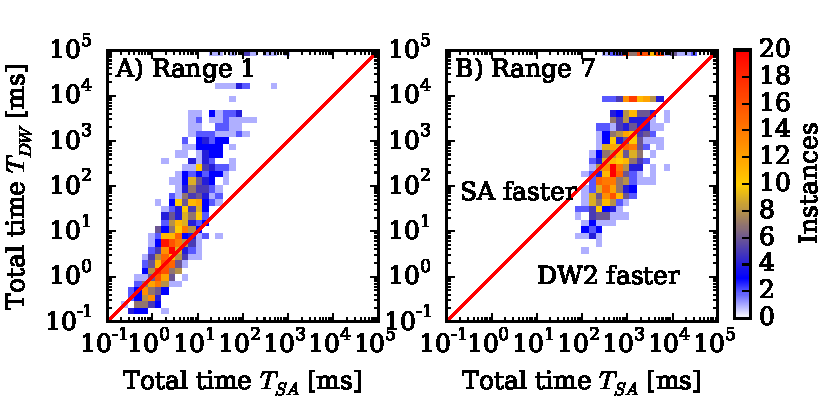
\includegraphics[width=0.95\columnwidth]{fig06.pdf} \label{fig:ratiosannealing}
\caption{{\bf Instance-by-instance comparison of annealing times.} Shown is a scatter plot of the pure annealing time for the DW2 compared to SA using an average over $16$ gauges (see \cite{SM}) on the DW2 for A) $r=1$ and B) $r=7$.  The color scale indicates the number of instances in each square. Instances below the diagonal red line are faster on the DW2, those above are faster using SA. Instances for which the DW2 did not find the solution with 10000 repetitions per gauge are shown at the top of the frame (no such instances were found for SA). 
%Panels C) and D)  show  wall-clock times using a single gauge on the DW2.
%Panels E) and F) show the wall-clock time for DW2 using $16$ gauges. $N=503$ in all cases. \red{Unless we discuss it in the text (currently not) we need to move wall-clock to SM.}
}
\label{fig:ratiosannealing}
\end{figure}
%%%%%%%%%
